\documentclass[12pt]{article}
\usepackage[margin=1in]{geometry}
\usepackage{enumitem}
\usepackage{titlesec}
\usepackage{parskip}
\usepackage{graphicx}
\usepackage{xcolor}
\usepackage{hyperref}
\usepackage{fontenc}

\title{\textbf{Boix 1999 RG Notes}\\
\large Boix, Carles. ``Setting the Rules of the Game: The Choice of Electoral Systems in Advanced Democracies'' [1999].\\
\textit{The American Political Science Review} 93(3): 609-624.}
\author{}
\date{}

\begin{document}

\maketitle

Because electoral systems are in part defined by the parties currently in power, there is a consistent dynamic whereby ruling parties alter electoral rules to maximize their own representation (and/or probability of winning outright). \underline{``As long as the electoral situation does not change substantially and the current rules serve the ruling parties well, the government has no incentives to modify the electoral regime. As soon as the electoral arena changes, however, the government considers altering the electoral system.''}

Electoral systems often change with the emergence of new parties (historically in 20th century, Socialist parties). If no mainstream party has a dominant standing in the current political sphere, then we should expect to see a shift to PR; however, if one party dominates (such that non-socialists can coalesce around a clear winner -- coordination problem here), then the majoritarian system will likely stand.

Open economies are drawn towards PR

\begin{center}
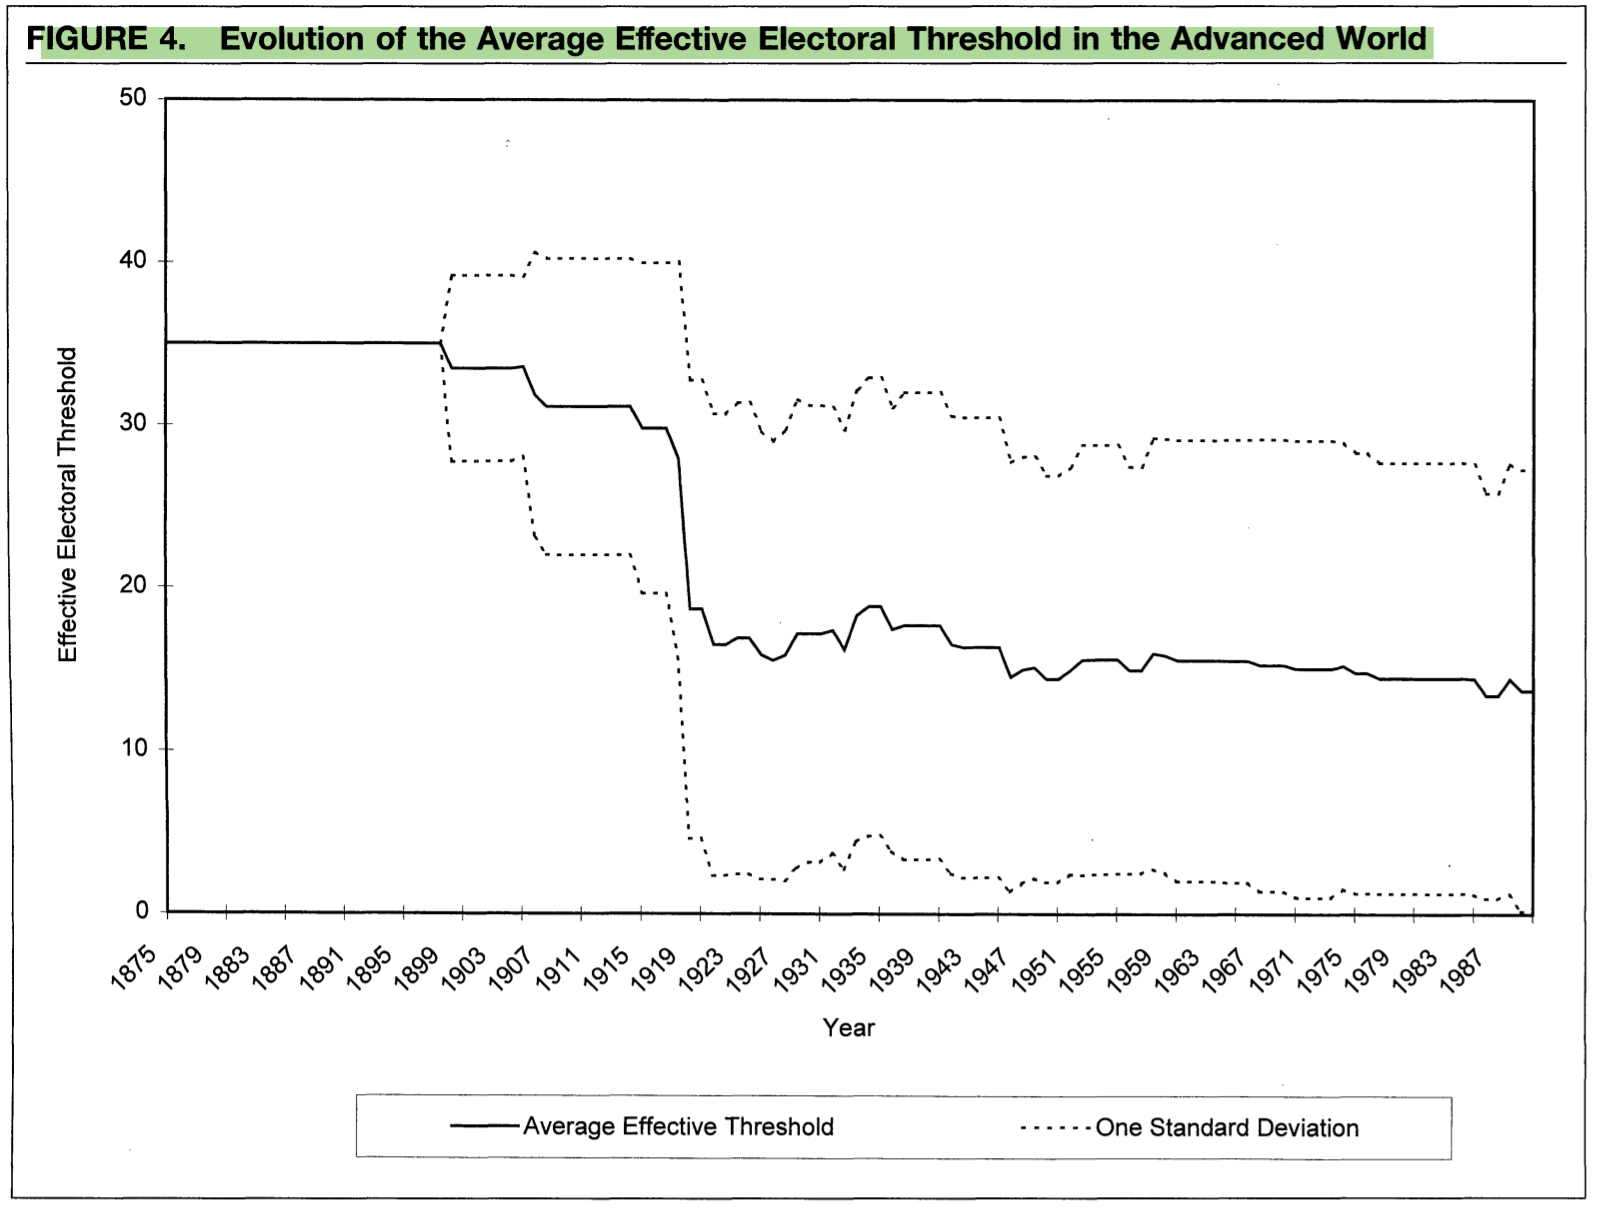
\includegraphics[width=0.85\textwidth]{figure-1.png}
\end{center}

[all quote follow]

Four different phenomena may lead to transformation of the political arena:

1) the extension of universal suffrage (Western Europe in the 1920s or new democratic nations in the postwar period);

2) the introduction of competitive elections (Eastern Europe and several African nations in the 1990s;

3) A massive political realignment among voters (the rise of socialism at the turn of the century or today's rise of protectionist parties, which would partly explain why France temporarily shifted to PR in 1986-88);

4) A high turnover in party organizations (France and Greece in this century)

\textbf{Compare to Harmel \textbackslash\{\}\& Janda 1994, who claim that party change is relatively intentional and endogenous; here, claim that political sphere change is largely exogenous at first, followed by endogenous responses}

\end{document}
